\documentclass{article}

\usepackage{amsmath} 
\usepackage{graphicx}
\usepackage{amsfonts}
\usepackage{array}

\begin{document}

\title{Catam 14.5 Cosmological Distances}
\date{September 2023}

\section{Distances and Time}
\subsection{Lookback Time}

The lookback time $t_L$ is the difference between the current age of the universe and the time at which the photons were emitted.

$$t_L = t_H \int_0^z \frac{dz'}{(1+z')E(z')}$$

With $t_H$ the Hubble time and $E(z) = \sqrt{\Omega_m(1+z)^3 + \Omega_k (1+z)^2 + \Omega_{\lambda}}$

\vspace{5mm}

Considering the Einstein-de-Sitter model Universe ($\Omega_m = 1,\ \Omega_\lambda = 0$) we can easily compute the age of the Universe.

$$t_0 = t_H \int_0^\infty (1+z')^{- \frac{5}{2}}dz' = - \frac{2}{3} t_H (1+z')^{- \frac{3}{2}} ]_0^\infty = \frac{2}{3}t_H$$


\subsubsection{Question 2}

We will consider four distinct models of the universe.
\begin{itemize}
	\item Einstein-de-Sitter universe ($\Omega_m = 1,\ \Omega_\lambda = 0$)
	\item Classical closed universe ($\Omega_m = 2,\ \Omega_\lambda =  0$)
	\item Baryon dominated low density universe ($\Omega_m = 0.04,\ \Omega_\lambda =  0$)
	\item Currently Popular universe ($\Omega_m = 0.27,\ \Omega_\lambda =  0.73$)
\end{itemize}

A program has been written to tabulate and graph results for lookback times in each of these models. It can be found in the "Code" section of the project.

\begin{table}[!h]
	\centering
	\begin{tabular}{ |c|cccc| }
		\hline
		Redshift & Einstein-de-Sitter & Classical closed & Baryon Dominated & Currently Popular \\ \hline \hline
		0.1      & 12.06762           & 11.80719         & 12.34083         & 12.68661          \\ \hline
		1.0      & 58.55965           & 52.94232         & 67.42440         & 76.28055          \\ \hline
		2.0      & 73.15351           & 64.55459         & 89.44977         & 101.87216         \\ \hline
		4.0      & 82.48464           & 71.64913         & 106.62361        & 119.34947         \\ \hline
		6.7      & 86.34735           & 74.50169         & 115.30207        & 126.735608        \\ \hline
		10000    & 90.87743           & 77.90534         & 128.53490        & 135.05773         \\ \hline
	\end{tabular}
	\caption{Lookback times in 100 million years for various redshifts}
\end{table}

Note that the last entry can be used as an approximation for the age of the universe as the redshift is so high the remaining part of the integral will be negligible.

\begin{figure}[ht!]
	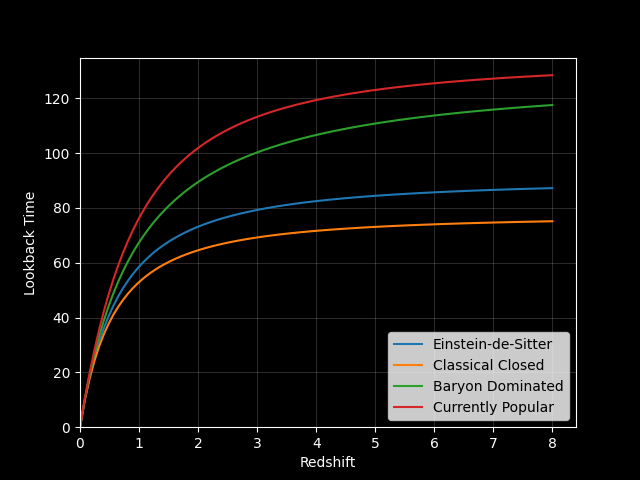
\includegraphics[width=\textwidth]{LookbackTimes.png}
	\caption{Lookback time graphed against redshift for various universes}\label{fig:my_label}
\end{figure}

\clearpage

\subsection{Distance Measures}

Considering the Einstein-de-Sitter model Universe ($\Omega_k = 0$) we get an expression for $D_A$ in:
$$D_A = \frac{D_C}{1+z} = \frac{D_H}{1+z} \int_0^z \frac{dz'}{E(z')} = \frac{D_H}{1+z}\int_0^z (1+z')^{-\frac{3}{2}}dz' = \frac{2D_H}{1+z} - \frac{2D_H}{(1+z)^{\frac{3}{2}}}$$

Finding stationary points:

$$\frac{d D_A}{dz} = - \frac{2D_H}{(1+z)^2} + \frac{3D_H}{(1+z)^{\frac{5}{2}}} = 0$$
$$\implies 2(1+z)^{\frac{1}{2}} = 3 \implies 4 + 4z = 9 \implies z = 1.25$$

Proving it is maxima:

$$\frac{d^2 D_A}{dz^2} = \frac{4D_H}{(1+z)^3} - \frac{15D_H}{2(1+z)^{\frac{7}{2}}}$$
$$\frac{d^2 D_A}{dz^2}|_{z=1.25} = D_H ( \frac{256}{729} - \frac{320}{729}) = -D_H \frac{64}{729} < 0$$

\subsubsection{Question 4}
A program has been written to compute $D_A$ and $D_L$ given a redshift and universe. It is also designed to plot the values of $D_A/D_H$ and $D_L/D_H$ against redshift. It can be found in the "Code" section of the project.

\begin{table}[!h]
	\centering
	\begin{tabular}{ |c|cc|cc|cc| }
		\hline
		         & Einstein  &           & Baryon    &           & Popular   &           \\
		Redshift & $D_A/D_H$ & $D_L/D_H$ & $D_A/D_H$ & $D_L/D_H$ & $D_A/D_H$ & $D_L/D_H$ \\ \hline \hline
		1.0      & 0.29260   & 1.17040   & 0.36969   & 1.47874   & 0.39244   & 1.56976   \\ \hline
		1.25     & 0.29600   & 1.49850   & 0.39401   & 1.99467   & 0.40981   & 2.07465   \\ \hline
		2.0      & 0.28148   & 2.53336   & 0.43112   & 3.88008   & 0.41366   & 3.72297   \\ \hline
		4.0      & 0.22089   & 5.52235   & 0.45001   & 11.25031  & 0.34575   & 8.64375   \\ \hline
	\end{tabular}
	\caption{Table of distance ratios according to redshift}
\end{table}

\begin{figure}[ht!]
	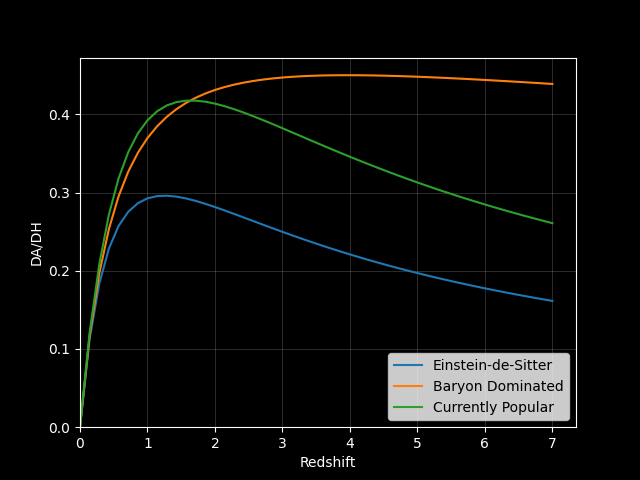
\includegraphics[width=\textwidth]{DADH.png}
	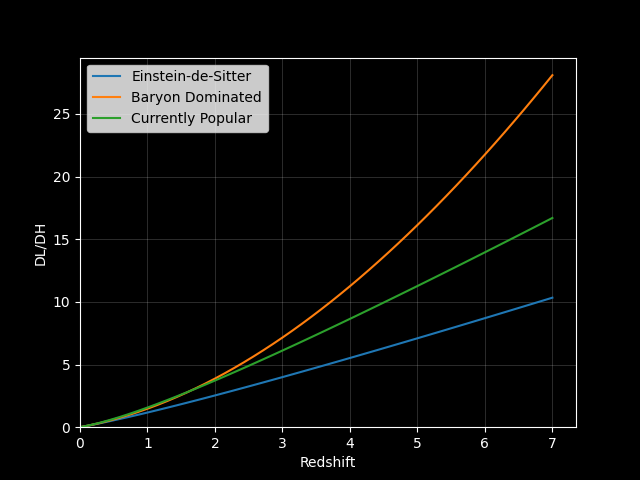
\includegraphics[width=\textwidth]{DLDH.png}
	\caption{Plots of $D_A/D_H$ and $D_L/D_H$ against redshift}
\end{figure}

\clearpage

\section{Comoving Volume}

\subsection{Uniform Comoving Distribution}

Finding $<V/V_{max}>$ we must average the population weighted according to $V/V_{max}$. It is clear that we should use the given formula for number of objects to create a probability distribution. We then see:

$$<V/V_{max}>\ = \frac{\int_0^\infty \Phi(L) \int_0^{V_{max(L)}} V/V_{max}dVdL}{\int_0^\infty \Phi(L) \int_0^{V_{max}(L)}dVdL}$$
$$= \frac{\int_0^\infty \Phi(L) \frac{1}{2}V_{max}dL}{\int_0^\infty \Phi(L) V_{max}dL} = \frac{1}{2}$$

[[Not exctly sure if this is right but we move come back to later i guess]]

\subsection{Computing $V/V_{max}$}
\subsubsection{Question 6}
A program has been written to compute $V$ and $V_{max}$ for arbitrary redshift $z$ and ratio between detected and minimum flux $f/f_0$. It works by computing the maximum redshift $z_0$
corresponding to a flux of $f_0$ by binary search and then using $z$ and $z_0$ along with the formulas provided to compute $D_C$ in each case, yielding $V$ and $V_{max}$.
The program can be found in the "Code" section of the project.

\vspace{5mm}
In an extension of this program it generates random numbers for $\Omega_m$, $z$ and $f/f_0$ with $z$ small and plots $(f/f_0)^{-\frac{3}{2}}$ against $V/V_{max}$ from the graph it is clear that in the euclidean limit they are directly proportional.

\begin{figure}[ht!]
	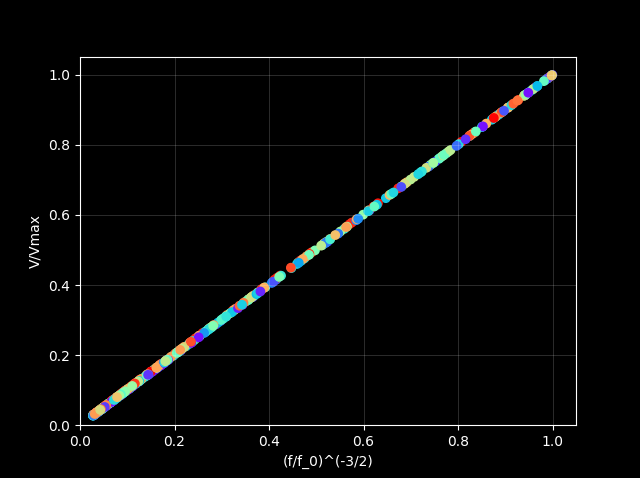
\includegraphics[width=\textwidth]{EuclideanLimit.png}
	\caption{Plot of $(f/f_0)^{-\frac{3}{2}}$ against $V/V_{max}$}
\end{figure}

\end{document}